\begin{itemize}
    \color{red}
    \item what is dense material tracking
    \item motivate the need for dense material tracking
    \begin{itemize}
        \item alternative to material surfaces
    \end{itemize}
    \item illustrate thin and thick scatterers
\end{itemize}

Usually tracking is done in as little material as possible to increase the resolution yield of the detector and the chance of detecting particles at all before they get "stopped". However, in some cases it is necessary to track particles through dense material. One example is track extension through a calorimeter to combine inner detector and muon system tracklets to improve the momentum resolution of high momentum muons at the interaction point.

One has two options to model the material in the calorimeter. Either virtual surfaces are inserted and the material of the calorimeter is projected on them similar to what is usually done in the inner detector. Or the material is modeled as a continous media. A volume-based approach also allows for continous energy loss and multiple scattering which can only be approximated by a surface-based approach. Ultimately, an experiment independet tracking software should be able to handle both cases.

While the surface-based approach is a long standing feature in ACTS, the volume-based approach was not implemented yet. This thesis aims to close this gap by implementing and validating volume-based material in ACTS.

This implementation focues on two interactions with the material, continuous energy loss and multiple scattering, which are described in the following sections. Aftwerwards, a reference with Geant4 is established and the implementation in ACTS is described. Finally, the performance of the implementation is evaluated.

\section{Modified Equation of Motion}

Continuous energy loss affects the trajectory of a particle and needs to be treated in the equation of motion. Secion \ref{sec:equation-of-motion} describes the equation of motion for a particle in a magnetic field. The equation of motion can be extended to include continuous energy loss by adding a term for the energy loss rate. The energy loss rate can be calculated using the Bethe-Bloch formula.

\begin{equation}
    \frac{d^2\vec{p}}{dt^2} = q \vec{v} \times \vec{B} - \frac{d\vec{p}}{dt}
\end{equation}

Apart from the energy loss, the particle's trajectory is also affected by multiple scattering. Multiple scattering is a random deflection of the particle's trajectory due to the Coulomb interaction with the material. Since this is a stochastic process which averages to no deflection over a large number of particles it has no effect on the average trajectory. However, it does affect the resolution of the track parameters which needs to be taken into account for the covariance transport.

\section{Covariance transport through thick scatterers}

\begin{itemize}
    \color{red}
    \item cannot be done by combining individual updates
    \item what about energy loss and its uncertainty?
\end{itemize}

While thin scatterers only incrase directional uncertainty, as the particle will pass through the scatterer before a positional uncertainty can build up, thick scatterers also increase the positional uncertainty while the particle passes through them.

\section{Toy Model}

\begin{itemize}
    \color{red}
    \item illustration
\end{itemize}

A toy model is used to simplify the implementation and validation of the volume-based material handling in ACTS. It consists of a box filled with dense material and a screen with some distance to the box. Muons are emitted from the left side of the box and their hits on the screen are recorded. This captures the essence of the problem without the complexity of a full detector simulation. Inside the dense material, the muons lose energy and scatter multiple times. The scattering not only affects the uncertainty of the direction but also the positional uncertainty on the screen. After passing the dense material, the muons are transported in a vacuum which should keep the uncertainty in direction unchanged but the positional uncertainty to further increase.

Note that this toy model does not include the magnetic field which is present in a real detector. The magnetic field bends the trajectory of the muons and potentially influences the covariance transport.

\section{Baseline with Geant4}

\begin{itemize}
    \color{red}
    \item setup, configuration and results
    \item special treatment to make multiple scattering work
    \item geant4 sim picture
    \item results for positional uncertainty on surface + fit
    \item results for energy loss + fit
\end{itemize}

A reference is established using Geant4 to compare it to the analytical solution which will be implemented in ACTS. Geant4 is a widely used particle transport simulation framework which is capable of simulating the interactions of particles with matter. It covers a wide range of interactions beyond the Bethe-Bloch energy loss and the Molière multiple scattering which are used in ACTS.

\begin{figure}[h]
    \centering
    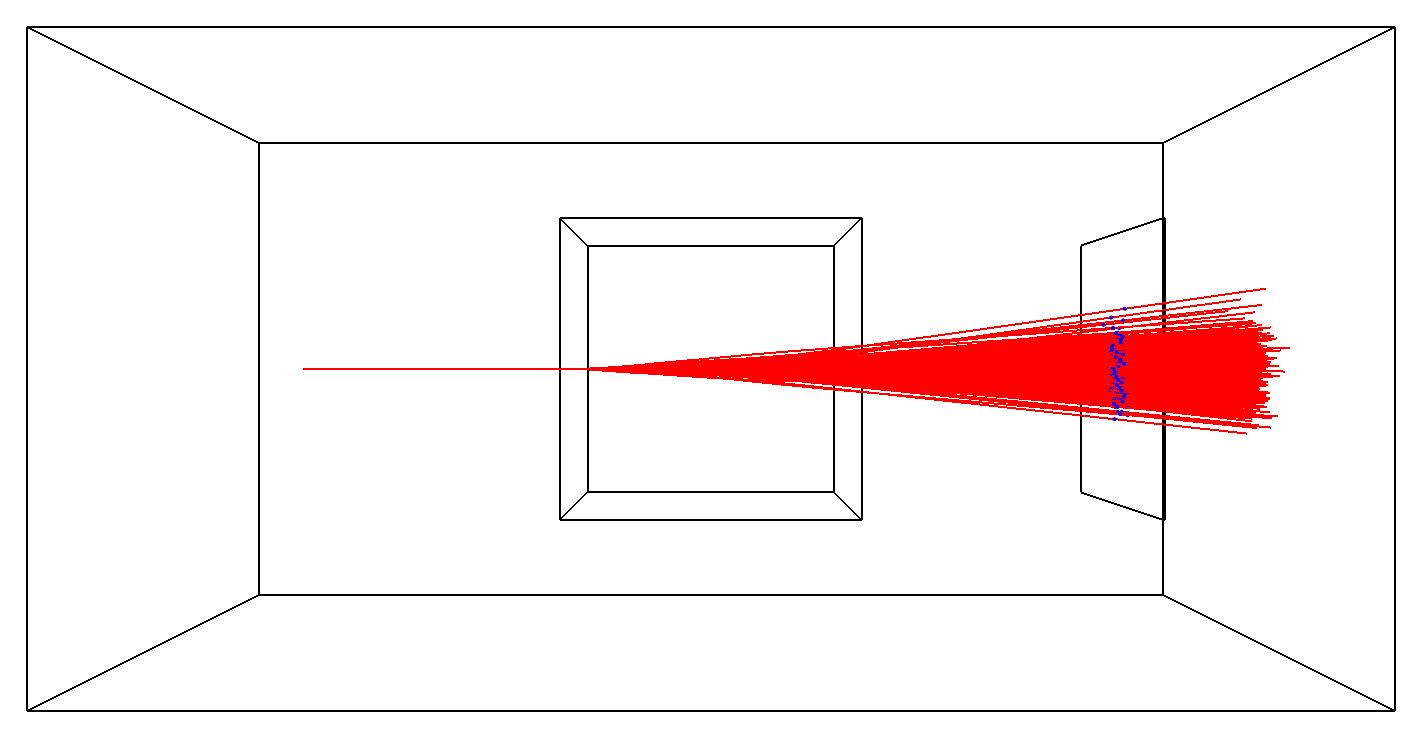
\includegraphics[width=0.8\textwidth]{parts/2_developments/08_dense-material-developments/figures/geant4_events.png}
    \caption{Event display showing 1000 muons passing through the toy geometry in Geant4. The outer box represents the world volume. The inner box represents the dense material. The muons are shown as red lines and originate from the left. The surface on the right represents the screen and the blue points are the hits on the screen.}
    \label{fig:dev/dense/geant4-events}
\end{figure}

\begin{figure}[h]
    \centering
    \includegraphics[width=1.0\textwidth]{parts/2_developments/08_dense-material-developments/figures/geant4_msc.pdf}
    \caption{The top row shows the density of the hits on the screen in local cartesian coordinates. For each column muons with a different energy are shown. The bottom row shows the hit positions of the local x coordinate on the screen with a fit to a Gaussian distribution.}
    \label{fig:dev/dense/geant4-msc}
\end{figure}

\section{First attempts with EigenStepper}

\begin{itemize}
    \color{red}
    \item EigenStepper dealt with integration of equations of motion but not multiple scattering
    \item Existing stepper abstraction did not allow for an easy integration of multiple scattering
    \item Simplification by removing stepper extension list and auctioneer
    \item Change of extension interface to allow for multiple scattering
    \item Link to the EigenStepper introduction and developments
\end{itemize}

ACTS already has volume material and an extension mechanism for the EigenStepper to deal with continuous energy loss. A natural first attempt was using this extension mechanism to deal with multiple scattering and get a first version of volume-based tracking.

Since steppers in ACTS primirily deal with Jacobian transport and transport the covariance only on demand, the additional angle and positional uncertainty due to multiple scattering cannot be simply added. To work around this, an additional covariance term was intoduced which is used to accumulate the multiple scattering uncertainty. This term is then added when the covariance is transported to the next surface.

While this approach worked, it was unsatisfactory because the multiple scattering contribution had to be recalculated at each step which is computationally inefficient. The extension mechanism needed a redesign to allow for multiple scattering to be calculated only once and then added to the covariance only when it is transported to the next surface. At the same time it was unclear how multiple extensions should cooperate on this additional covariance. This bigger architectural change of ACTS was not directly attempted and this first solution was only a proof of concept and kept in a separate branch.

\begin{figure}[h]
    \centering
    \includegraphics[width=1.0\textwidth]{parts/2_developments/08_dense-material-developments/figures/eloss_cmp.pdf}
    \caption{A comparison of the energy loss computed by ACTS and Geant4 for muons with different energies. The vertical bars represent the uncertainty of the energy loss.}
    \label{fig:dev/dense/eloss_cmp}
\end{figure}

\section{SympyStepper}

\begin{itemize}
    \color{red}
    \item Alternative to EigenStepper with explicit math expressions
    \begin{itemize}
        \item avoids extension by having different RK4 integration routines. removes one layer of abstraction
    \end{itemize}
    \item Link to the SympyStepper introduction and developments
\end{itemize}

The SympyStepper is a new stepper implementation in ACTS which uses symbolic math expressions and transforms them into code.

As this is a new implementation we could avoid the extension mechanism of the EigenStepper completely and think of a way to integrate dense material from the beginning. The extended equation of motion to deal with continous energy loss was implemented in a separate routine which is called internally by the SympyStepper when the particle is in dense material. So instead of trying to generalize this we just enumerate the two cases we are aware of: vacuum and dense material.

\section{Performance}

\begin{itemize}
    \color{red}
    \item physics performance comparison of Geant4, EigenStepper and SympyStepper
    \item CPU performance comparison of EigenStepper and SympyStepper with and without dense material
\end{itemize}
